\section{The symmetric wavelet transform}
\label{sec:transform}

The transform is where WSQ gets its compression power. It does not reduce the amount of data
(it maps $XY$ samples to $XY$ coefficients) but it concentrates the image's energy: after the
transform, most coefficients are close to zero and the few large ones describe the ridge
pattern. This section builds the transform in four steps: a two-channel filter bank in one
dimension, the symmetric extension that makes it work on finite signals, the separable
two-dimensional version, and the particular cascade of 64 subbands the standard prescribes.

\subsection{The two-channel filter bank}

Figure~\ref{fig:filterbank} shows the building block (Annex A.2.1 of the specification). The
input $x$ goes through a lowpass filter $h_0$ and a highpass filter $h_1$, and each output is
\emph{decimated}: only every other sample is kept. The two half-length signals $a_0$ and $a_1$
are the \emph{subbands}. To reconstruct, each subband is \emph{upsampled} (a zero is inserted
between consecutive samples), filtered by a synthesis filter $f_0$ or $f_1$, and the two results
are added. With
\begin{equation*}
  (x * h)(k) = \sum_{n} x(n)\,h(k-n), \qquad
  ({\downarrow} y)(k) = y(2k), \qquad
  ({\uparrow} a)(n) = \begin{cases} a(n/2) & n \text{ even},\\ 0 & n \text{ odd},\end{cases}
\end{equation*}
the analysis bank computes $a_i = {\downarrow}(x * h_i)$ and the synthesis bank
$\hat x = f_0 * ({\uparrow} a_0) + f_1 * ({\uparrow} a_1)$.

\begin{figure}[ht]
  \centering
  \begin{tikzpicture}[node distance=4mm and 6mm,
    f/.style={box,minimum width=9mm,font=\small},
    s/.style={box,minimum width=7mm,font=\small}]
  \node[font=\small] (x) {$x$};
  \coordinate[right=5mm of x] (fork);
  \node[f,above right=4mm and 6mm of fork] (h1) {$h_1$};
  \node[f,below right=4mm and 6mm of fork] (h0) {$h_0$};
  \node[s,right=of h1] (d1) {$\downarrow 2$};
  \node[s,right=of h0] (d0) {$\downarrow 2$};
  \node[s,right=11mm of d1] (u1) {$\uparrow 2$};
  \node[s,right=11mm of d0] (u0) {$\uparrow 2$};
  \node[f,right=of u1] (f1) {$f_1$};
  \node[f,right=of u0] (f0) {$f_0$};
  \node[op,right=8mm of $(f1)!0.5!(f0)$] (sum) {$+$};
  \node[font=\small,right=5mm of sum] (xh) {$\hat x$};
  \draw (x) -- (fork);
  \draw[->] (fork) |- (h1);
  \draw[->] (fork) |- (h0);
  \draw[->] (h1) -- (d1);
  \draw[->] (h0) -- (d0);
  \draw[->] (d1) -- node[above,font=\small] {$a_1$} (u1);
  \draw[->] (d0) -- node[above,font=\small] {$a_0$} (u0);
  \draw[->] (u1) -- (f1);
  \draw[->] (u0) -- (f0);
  \draw[->] (f1) -| (sum);
  \draw[->] (f0) -| (sum);
  \draw[->] (sum) -- (xh);
  \node[font=\footnotesize,above=7mm of $(h1)!0.5!(d1)$] {analysis};
  \node[font=\footnotesize,above=7mm of $(u1)!0.5!(f1)$] {synthesis};
\end{tikzpicture}

  \caption{Two-channel subband coder. With the right filters the output equals the input.}
  \label{fig:filterbank}
\end{figure}

Decimation discards half the samples of each branch, so each subband on its own is aliased.
The synthesis filters are chosen so that the aliasing of the two branches cancels and
$\hat x = x$ exactly (\emph{perfect reconstruction}). WSQ uses the \emph{anti-aliasing
relations}
\begin{equation}
  f_0(n) = (-1)^n\, h_1(n-1), \qquad f_1(n) = (-1)^{n-1}\, h_0(n-1),
  \label{eq:antialias}
\end{equation}
which make the aliasing terms cancel identically. Together with a biorthogonality condition
between $h_0$ and $h_1$ they give perfect reconstruction. Because of
Equation~\eqref{eq:antialias}, a WSQ file only carries the analysis filters, and only half of
each, since they are symmetric.

\subsection{Linear-phase filters}

WSQ allows two families of symmetric (linear-phase) filter banks (Annex A.2.1.1).
\begin{description}[leftmargin=0pt]
  \item[Whole-sample symmetric (WS) banks] have odd-length filters. The lowpass filter $h_0$
    is symmetric about $0$, $h_0(-n) = h_0(n)$, and runs from $-r_0$ to $r_0$ (length
    $L_0 = 2r_0+1$). The highpass filter $h_1$ is symmetric about $-1$,
    $h_1(-1-n) = h_1(n-1)$, and runs from $-1-r_1$ to $-1+r_1$ (length $L_1 = 2r_1+1$).
    The file carries $h_0(0),\dots,h_0(r_0)$ and $h_1(-1),\dots,h_1(r_1-1)$.
  \item[Half-sample symmetric (HS) banks] have even-length filters, both centred at
    $-\tfrac12$ and running from $-r_i$ to $r_i - 1$ (length $L_i = 2r_i$). The lowpass
    filter is symmetric, $h_0(-1-n) = h_0(n)$, and the highpass filter antisymmetric,
    $h_1(-1-n) = -h_1(n)$. The file carries $h_i(0),\dots,h_i(r_i-1)$.
\end{description}
Decoders must accept lengths up to 31 (WS) and 32 (HS). Encoder number two uses the WS bank
of Table~\ref{tab:filters}, a 9-tap lowpass and a 7-tap highpass filter from the family of
Cohen, Daubechies and Feauveau that Antonini et al.\ introduced for image coding
\cite{antonini1992}; JPEG~2000 later adopted the same pair. The specification also gives
their exact values: with
\begin{equation*}
  A = \Bigl(\frac{-14\sqrt{15}+63}{1080\sqrt{15}}\Bigr)^{1/3},\quad
  B = \Bigl(\frac{-14\sqrt{15}-63}{1080\sqrt{15}}\Bigr)^{1/3},\quad
  x_1 = A + B - \tfrac16,\quad
  x_2 = -\tfrac{A+B}{2} - \tfrac16 + \mathrm{i}\,\tfrac{\sqrt3}{2}(A-B),
\end{equation*}
(real cube roots), the taps are
\begin{align*}
  h_0(0)     &= -5\sqrt2\,x_1\,(48|x_2|^2 - 16\,\mathrm{Re}\,x_2 + 3)/32, &
  h_1(-1)    &= \sqrt2\,(6x_1-1)/(16x_1),\\
  h_0(\pm1)  &= -5\sqrt2\,x_1\,(8|x_2|^2 - \mathrm{Re}\,x_2)/8, &
  h_1(-2) = h_1(0) &= -\sqrt2\,(16x_1-1)/(64x_1),\\
  h_0(\pm2)  &= -5\sqrt2\,x_1\,(4|x_2|^2 + 4\,\mathrm{Re}\,x_2 - 1)/16, &
  h_1(-3) = h_1(1) &= \sqrt2\,(2x_1+1)/(32x_1),\\
  h_0(\pm3)  &= -5\sqrt2\,x_1\,\mathrm{Re}\,x_2/8, &
  h_1(-4) = h_1(2) &= -\sqrt2/(64x_1),\\
  h_0(\pm4)  &= -5\sqrt2\,x_1/64.
\end{align*}
The lowpass taps add up to $\sqrt2$ and the highpass taps to zero.

\begin{table}[ht]
  \centering\small
  \begin{tabular}{@{}lr@{\qquad}lr@{}}
    \toprule
    tap & value & tap & value \\
    \midrule
    $h_0(0)$       &  0.852698679009403 & $h_1(-1)$       &  0.788485616405664 \\
    $h_0(\pm1)$    &  0.377402855612654 & $h_1(-2),h_1(0)$ & $-0.418092273222212$ \\
    $h_0(\pm2)$    & $-0.110624404418423$ & $h_1(-3),h_1(1)$ & $-0.040689417609558$ \\
    $h_0(\pm3)$    & $-0.023849465019380$ & $h_1(-4),h_1(2)$ &  0.064538882628938 \\
    $h_0(\pm4)$    &  0.037828455506995 & & \\
    \bottomrule
  \end{tabular}
  \caption{The analysis filters of encoder number two (Part 3, Table 1).}
  \label{tab:filters}
\end{table}

\subsection{Finite signals: symmetric extension}
\label{sec:extension}

A filter bank is defined on infinite signals, while an image row has $N_0$ samples. Treating
the samples outside the row as zero, or wrapping the row around periodically, creates a jump
at the borders. A jump has energy at every frequency, so it would fill the highpass subbands
with large coefficients that carry no information about the fingerprint.

WSQ mirrors the signal at its ends instead (Annex A.2.2), as in Figure~\ref{fig:extension}.
With a WS bank the row is reflected about its first and last samples without repeating them,
which gives a signal of period $2N_0-2$; with an HS bank it is reflected about the half-sample
points $-\tfrac12$ and $N_0-\tfrac12$, repeating the end samples, which gives period $2N_0$.
The mirrored signal is continuous at the borders. Moreover, a symmetric signal filtered by a
symmetric filter is again symmetric, so the subbands of the extended signal are themselves
symmetric and periodic, and only a non-redundant part of each needs to be stored. That part has
$\ceil{N_0/2}$ samples for the lowpass subband and $\floor{N_0/2}$ for the highpass one:
$N_0$ samples in, $N_0$ coefficients out. The specification calls this the \emph{symmetric
wavelet transform} (SWT) \cite{brislawn1992}.

\begin{figure}[ht]
  \centering
  % Generated by tools/gen_figures.py; do not edit by hand.
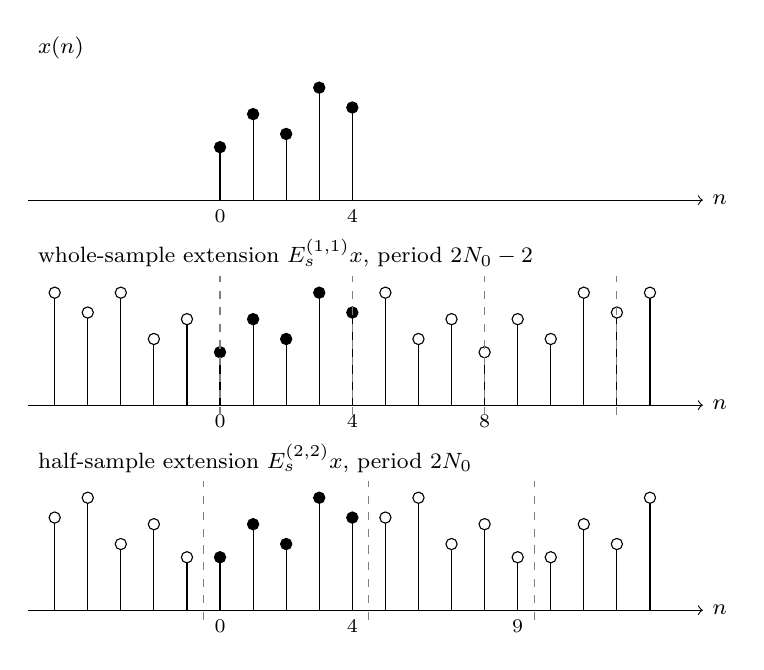
\begin{tikzpicture}[x=0.42cm,y=0.42cm]
  \draw[->] (-5.8,-0.0) -- (14.6,-0.0) node[right,font=\footnotesize] {$n$};
  \node[anchor=west,font=\footnotesize] at (-5.8,4.6) {$x(n)$};
  \draw (0,-0.0) -- (0,1.6);
  \fill[black,draw=black] (0,1.6) circle (0.17);
  \draw (1,-0.0) -- (1,2.6);
  \fill[black,draw=black] (1,2.6) circle (0.17);
  \draw (2,-0.0) -- (2,2.0);
  \fill[black,draw=black] (2,2.0) circle (0.17);
  \draw (3,-0.0) -- (3,3.4);
  \fill[black,draw=black] (3,3.4) circle (0.17);
  \draw (4,-0.0) -- (4,2.8);
  \fill[black,draw=black] (4,2.8) circle (0.17);
  \node[below,font=\scriptsize] at (0,-0.0) {0};
  \node[below,font=\scriptsize] at (4,-0.0) {4};
  \draw[->] (-5.8,-6.2) -- (14.6,-6.2) node[right,font=\footnotesize] {$n$};
  \node[anchor=west,font=\footnotesize] at (-5.8,-1.6000000000000005) {whole-sample extension $E_s^{(1,1)}x$, period $2N_0-2$};
  \draw (-5,-6.2) -- (-5,-2.8000000000000003);
  \fill[white,draw=black] (-5,-2.8000000000000003) circle (0.17);
  \draw (-4,-6.2) -- (-4,-3.4000000000000004);
  \fill[white,draw=black] (-4,-3.4000000000000004) circle (0.17);
  \draw (-3,-6.2) -- (-3,-2.8000000000000003);
  \fill[white,draw=black] (-3,-2.8000000000000003) circle (0.17);
  \draw (-2,-6.2) -- (-2,-4.2);
  \fill[white,draw=black] (-2,-4.2) circle (0.17);
  \draw (-1,-6.2) -- (-1,-3.6);
  \fill[white,draw=black] (-1,-3.6) circle (0.17);
  \draw (0,-6.2) -- (0,-4.6);
  \fill[black,draw=black] (0,-4.6) circle (0.17);
  \draw (1,-6.2) -- (1,-3.6);
  \fill[black,draw=black] (1,-3.6) circle (0.17);
  \draw (2,-6.2) -- (2,-4.2);
  \fill[black,draw=black] (2,-4.2) circle (0.17);
  \draw (3,-6.2) -- (3,-2.8000000000000003);
  \fill[black,draw=black] (3,-2.8000000000000003) circle (0.17);
  \draw (4,-6.2) -- (4,-3.4000000000000004);
  \fill[black,draw=black] (4,-3.4000000000000004) circle (0.17);
  \draw (5,-6.2) -- (5,-2.8000000000000003);
  \fill[white,draw=black] (5,-2.8000000000000003) circle (0.17);
  \draw (6,-6.2) -- (6,-4.2);
  \fill[white,draw=black] (6,-4.2) circle (0.17);
  \draw (7,-6.2) -- (7,-3.6);
  \fill[white,draw=black] (7,-3.6) circle (0.17);
  \draw (8,-6.2) -- (8,-4.6);
  \fill[white,draw=black] (8,-4.6) circle (0.17);
  \draw (9,-6.2) -- (9,-3.6);
  \fill[white,draw=black] (9,-3.6) circle (0.17);
  \draw (10,-6.2) -- (10,-4.2);
  \fill[white,draw=black] (10,-4.2) circle (0.17);
  \draw (11,-6.2) -- (11,-2.8000000000000003);
  \fill[white,draw=black] (11,-2.8000000000000003) circle (0.17);
  \draw (12,-6.2) -- (12,-3.4000000000000004);
  \fill[white,draw=black] (12,-3.4000000000000004) circle (0.17);
  \draw (13,-6.2) -- (13,-2.8000000000000003);
  \fill[white,draw=black] (13,-2.8000000000000003) circle (0.17);
  \node[below,font=\scriptsize] at (0,-6.2) {0};
  \node[below,font=\scriptsize] at (4,-6.2) {4};
  \node[below,font=\scriptsize] at (8,-6.2) {8};
  \draw[dashed,gray] (0,-6.5) -- (0,-2.3000000000000003);
  \draw[dashed,gray] (4,-6.5) -- (4,-2.3000000000000003);
  \draw[dashed,gray] (8,-6.5) -- (8,-2.3000000000000003);
  \draw[dashed,gray] (12,-6.5) -- (12,-2.3000000000000003);
  \draw[->] (-5.8,-12.4) -- (14.6,-12.4) node[right,font=\footnotesize] {$n$};
  \node[anchor=west,font=\footnotesize] at (-5.8,-7.800000000000001) {half-sample extension $E_s^{(2,2)}x$, period $2N_0$};
  \draw (-5,-12.4) -- (-5,-9.600000000000001);
  \fill[white,draw=black] (-5,-9.600000000000001) circle (0.17);
  \draw (-4,-12.4) -- (-4,-9.0);
  \fill[white,draw=black] (-4,-9.0) circle (0.17);
  \draw (-3,-12.4) -- (-3,-10.4);
  \fill[white,draw=black] (-3,-10.4) circle (0.17);
  \draw (-2,-12.4) -- (-2,-9.8);
  \fill[white,draw=black] (-2,-9.8) circle (0.17);
  \draw (-1,-12.4) -- (-1,-10.8);
  \fill[white,draw=black] (-1,-10.8) circle (0.17);
  \draw (0,-12.4) -- (0,-10.8);
  \fill[black,draw=black] (0,-10.8) circle (0.17);
  \draw (1,-12.4) -- (1,-9.8);
  \fill[black,draw=black] (1,-9.8) circle (0.17);
  \draw (2,-12.4) -- (2,-10.4);
  \fill[black,draw=black] (2,-10.4) circle (0.17);
  \draw (3,-12.4) -- (3,-9.0);
  \fill[black,draw=black] (3,-9.0) circle (0.17);
  \draw (4,-12.4) -- (4,-9.600000000000001);
  \fill[black,draw=black] (4,-9.600000000000001) circle (0.17);
  \draw (5,-12.4) -- (5,-9.600000000000001);
  \fill[white,draw=black] (5,-9.600000000000001) circle (0.17);
  \draw (6,-12.4) -- (6,-9.0);
  \fill[white,draw=black] (6,-9.0) circle (0.17);
  \draw (7,-12.4) -- (7,-10.4);
  \fill[white,draw=black] (7,-10.4) circle (0.17);
  \draw (8,-12.4) -- (8,-9.8);
  \fill[white,draw=black] (8,-9.8) circle (0.17);
  \draw (9,-12.4) -- (9,-10.8);
  \fill[white,draw=black] (9,-10.8) circle (0.17);
  \draw (10,-12.4) -- (10,-10.8);
  \fill[white,draw=black] (10,-10.8) circle (0.17);
  \draw (11,-12.4) -- (11,-9.8);
  \fill[white,draw=black] (11,-9.8) circle (0.17);
  \draw (12,-12.4) -- (12,-10.4);
  \fill[white,draw=black] (12,-10.4) circle (0.17);
  \draw (13,-12.4) -- (13,-9.0);
  \fill[white,draw=black] (13,-9.0) circle (0.17);
  \node[below,font=\scriptsize] at (0,-12.4) {0};
  \node[below,font=\scriptsize] at (4,-12.4) {4};
  \node[below,font=\scriptsize] at (9,-12.4) {9};
  \draw[dashed,gray] (-0.5,-12.700000000000001) -- (-0.5,-8.5);
  \draw[dashed,gray] (4.5,-12.700000000000001) -- (4.5,-8.5);
  \draw[dashed,gray] (9.5,-12.700000000000001) -- (9.5,-8.5);
\end{tikzpicture}

  \caption{A signal of $N_0 = 5$ samples (filled) and its two symmetric extensions (hollow
  samples are mirror images). Dashed lines mark the centres of symmetry.}
  \label{fig:extension}
\end{figure}

In formulas, let $\tilde x$ be the extended signal. For a WS bank, with period $P = 2N_0-2$
and $u = n \bmod P$ taken in $[0, P)$,
\begin{equation}
  \tilde x(n) = x\bigl(u\bigr) \text{ if } u < N_0, \qquad \tilde x(n) = x\bigl(P-u\bigr) \text{ otherwise};
  \label{eq:wsext}
\end{equation}
for an HS bank, with $P = 2N_0$, the second case reads $x(P-1-u)$. (A one-sample signal
extends to a constant.) The subbands are
\begin{equation}
  a_0(k) = \sum_j h_0(j)\,\tilde x(2k-j), \quad 0 \le k < \ceil{N_0/2}, \qquad
  a_1(k) = \sum_j h_1(j)\,\tilde x(2k-j), \quad 0 \le k < \floor{N_0/2}.
  \label{eq:analysis}
\end{equation}
With the WS bank of Table~\ref{tab:filters}, $a_0(k)$ is a weighted average centred on the
even sample $2k$, and $a_1(k)$ a difference centred on the odd sample $2k+1$ (because $h_1$ is
centred at $-1$). Algorithm~\ref{alg:analysis} spells this out.

\begin{algorithm}[ht]
  \caption{One-dimensional symmetric wavelet analysis.}
  \label{alg:analysis}
  \begin{algorithmic}[1]
    \Require $x(0),\dots,x(N_0-1)$; analysis filters $h_0, h_1$; bank type WS or HS
    \Ensure $a_0$ with $\ceil{N_0/2}$ values, $a_1$ with $\floor{N_0/2}$ values
    \Function{Ext}{$n$} \Comment{index into $x$ of sample $n$ of the extension}
      \If{$N_0 = 1$} \Return $0$ \EndIf
      \If{WS} \State $P \gets 2N_0 - 2$;\ $u \gets n \bmod P$;\ \Return $u$ \textbf{if} $u < N_0$ \textbf{else} $P - u$
      \Else \State $P \gets 2N_0$;\ $u \gets n \bmod P$;\ \Return $u$ \textbf{if} $u < N_0$ \textbf{else} $P - 1 - u$
      \EndIf
    \EndFunction
    \For{$k \gets 0$ \textbf{to} $\ceil{N_0/2}-1$}
      \State $a_0(k) \gets \sum_{j} h_0(j)\; x\bigl(\Call{Ext}{2k - j}\bigr)$ \Comment{$j$ over the taps of $h_0$}
    \EndFor
    \For{$k \gets 0$ \textbf{to} $\floor{N_0/2}-1$}
      \State $a_1(k) \gets \sum_{j} h_1(j)\; x\bigl(\Call{Ext}{2k - j}\bigr)$
    \EndFor
  \end{algorithmic}
\end{algorithm}

\subsection{Synthesis}

To invert, the decoder rebuilds the full periodic subbands $b_0$ and $b_1$ from the stored
halves using their symmetries (Annex A.2.2.1 and its Table A.1), then applies the synthesis
bank. The symmetries follow from those of the extension and the filters, and they lead to
simple index maps. Let $\rho_0 = \ceil{N_0/2}$ and $\rho_1 = \floor{N_0/2}$ be the stored
lengths.
\begin{itemize}
  \item WS bank: both subbands have period $P = N_0 - 1$. With $u = k \bmod P$,
    \[
      b_0(k) = a_0\bigl(\min(u,\,P-u)\bigr), \qquad b_1(k) = a_1\bigl(\min(u,\,P-1-u)\bigr).
    \]
    The lowpass subband is symmetric about $0$ and the highpass one about $-\tfrac12$.
  \item HS bank: both subbands have period $N_0$. With $u = k \bmod N_0$ and $v = N_0-1-u$,
    \[
      b_0(k) = a_0\bigl(\min(u,v)\bigr), \qquad
      b_1(k) = \begin{cases} a_1(u) & u < v,\\ -a_1(v) & u > v,\\ 0 & u = v. \end{cases}
    \]
    The highpass subband is antisymmetric, and when $N_0$ is odd its centre sample is zero,
    which is why only $(N_0-1)/2$ values are stored.
\end{itemize}
The reconstruction is then
\begin{equation}
  x(n) = \sum_{k} f_0(n-2k)\,b_0(k) + \sum_{k} f_1(n-2k)\,b_1(k), \qquad 0 \le n < N_0,
  \label{eq:synthesis}
\end{equation}
where the sums run over the $k$ for which the filter tap exists. Algorithm~\ref{alg:synthesis}
writes it out. These index maps are equivalent to the extension operators of the
specification; implemented as written, Algorithms~\ref{alg:analysis} and~\ref{alg:synthesis}
reconstruct random signals of every length from 1 to 101 to within $10^{-13}$, with the
encoder number two filters and with the Haar HS bank.

\begin{algorithm}[ht]
  \caption{One-dimensional symmetric wavelet synthesis.}
  \label{alg:synthesis}
  \begin{algorithmic}[1]
    \Require $a_0$ ($\rho_0$ values), $a_1$ ($\rho_1$ values); synthesis filters $f_0, f_1$ from Eq.~\eqref{eq:antialias}
    \Ensure $x(0),\dots,x(N_0-1)$, with $N_0 = \rho_0 + \rho_1$
    \Function{B$_0$}{$k$}
      \If{WS} \If{$N_0 = 1$} \Return $a_0(0)$ \EndIf
        \State $P \gets N_0 - 1$;\ $u \gets k \bmod P$;\ \Return $a_0(\min(u, P-u))$
      \Else \State $u \gets k \bmod N_0$;\ \Return $a_0(\min(u, N_0-1-u))$
      \EndIf
    \EndFunction
    \Function{B$_1$}{$k$}
      \If{WS} \State $P \gets N_0 - 1$;\ $u \gets k \bmod P$;\ \Return $a_1(\min(u, P-1-u))$
      \Else \State $u \gets k \bmod N_0$;\ $v \gets N_0-1-u$
        \If{$u < v$} \Return $a_1(u)$ \ElsIf{$u > v$} \Return $-a_1(v)$ \Else\ \Return $0$ \EndIf
      \EndIf
    \EndFunction
    \For{$n \gets 0$ \textbf{to} $N_0-1$}
      \State $x(n) \gets \sum_{t:\ n-t \text{ even}} f_0(t)\,\Call{B$_0$}{(n-t)/2}$
      \State $x(n) \gets x(n) + \sum_{t:\ n-t \text{ even}} f_1(t)\,\Call{B$_1$}{(n-t)/2}$ \Comment{skipped when $\rho_1 = 0$}
    \EndFor
  \end{algorithmic}
\end{algorithm}

\subsection{Two dimensions}

Images are transformed separably (Annex A.2.3): every row is passed through the
one-dimensional SWT, and then every column of the result. The rows yield a lowpass half on
the left and a highpass half on the right; the columns split each half again into a top and a
bottom part. One level therefore produces four subbands (Figure~\ref{fig:twodim}). The
specification names them $a_{ij}$, where $i$ is the filter applied along the rows (horizontal
direction) and $j$ the one applied along the columns: $a_{10}$ is highpass horizontally and
lowpass vertically, so it responds to vertical edges. The inverse transform does the opposite,
columns first and rows second.

\begin{figure}[ht]
  \centering
  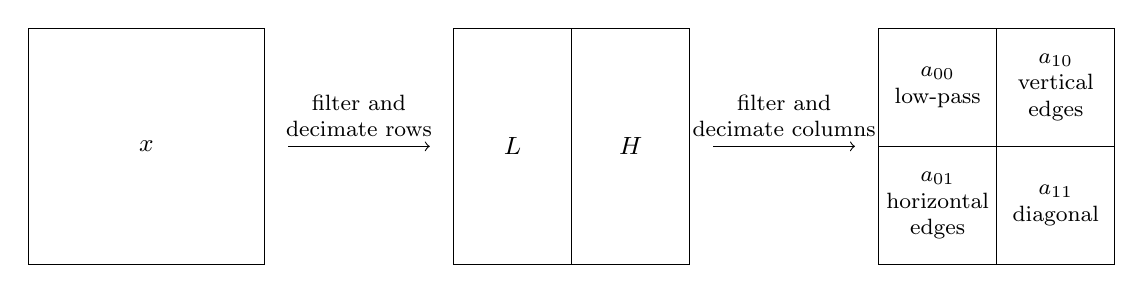
\begin{tikzpicture}[x=1cm,y=-1cm,font=\small]
  % input
  \draw (0,0) rectangle (3,3);
  \node at (1.5,1.5) {$x$};
  \draw[->] (3.3,1.5) -- node[above,font=\footnotesize,align=center] {filter and\\decimate rows} (5.1,1.5);
  % after rows
  \draw (5.4,0) rectangle (8.4,3);
  \draw (6.9,0) -- (6.9,3);
  \node at (6.15,1.5) {$L$};
  \node at (7.65,1.5) {$H$};
  \draw[->] (8.7,1.5) -- node[above,font=\footnotesize,align=center] {filter and\\decimate columns} (10.5,1.5);
  % after columns
  \draw (10.8,0) rectangle (13.8,3);
  \draw (12.3,0) -- (12.3,3) (10.8,1.5) -- (13.8,1.5);
  \node[align=center,font=\footnotesize] at (11.55,0.75) {$a_{00}$\\low-pass};
  \node[align=center,font=\footnotesize] at (13.05,0.75) {$a_{10}$\\vertical\\edges};
  \node[align=center,font=\footnotesize] at (11.55,2.25) {$a_{01}$\\horizontal\\edges};
  \node[align=center,font=\footnotesize] at (13.05,2.25) {$a_{11}$\\diagonal};
\end{tikzpicture}

  \caption{One level of the separable two-dimensional transform.}
  \label{fig:twodim}
\end{figure}

\subsection{Spectral inversion}
\label{sec:inversion}

WSQ applies the filter bank again to some of the subbands it produces. Splitting the lowpass
subband again is straightforward, but splitting a highpass subband involves a subtlety. A
cosine of frequency $\omega$ sampled at the even positions becomes
$\cos(2\omega k) = \cos\bigl((2\pi - 2\omega)k\bigr)$, so decimation maps the band
$[\pi/2, \pi]$ onto $[0, \pi]$ \emph{in reverse}: the highest frequencies of the original end up
at the lowest frequencies of the subband. The highpass subband is spectrally mirrored.
If it is split again, its lowpass half holds the original frequencies near $\pi$, and its
highpass half those near $\pi/2$.

The specification orders subbands by the original frequency they represent, from the top left
(lowest) to the bottom right (highest). A mirrored region must therefore store the highpass
output of its split \emph{first}. Figure~\ref{fig:inversion} shows two levels in one
dimension: the four bands, in increasing frequency, have filter paths $00$, $01$, $11$ and $10$,
a Gray code. In general, a band's position along an axis is obtained from its filter path
(0 for lowpass, 1 for highpass) by a running exclusive-or, and the
\emph{Filter Bank Path} table of Figure A.5 of the specification follows this rule.

\begin{figure}[ht]
  \centering
  \begin{tikzpicture}[x=3.2cm,y=-1cm,font=\small]
  % a band from #1 to #2 on row #3, label #4, spectrum orientation #5 (1 normal, -1 mirrored)
  \newcommand{\band}[5]{%
    \draw (#1,#3) rectangle (#2,#3+0.8);
    \node at ({(#1+#2)/2},#3+0.27) {#4};
    \ifnum#5=1
      \draw[->,gray] ({#1+0.12*(#2-#1)},#3+0.6) -- ({#2-0.12*(#2-#1)},#3+0.6);
    \else
      \draw[<-,gray] ({#1+0.12*(#2-#1)},#3+0.6) -- ({#2-0.12*(#2-#1)},#3+0.6);
    \fi}
  \band{0}{4}{0}{$x$}{1}
  \band{0}{2}{1.6}{$L$}{1}
  \band{2}{4}{1.6}{$H$, mirrored}{-1}
  \band{0}{1}{3.2}{$LL$\quad path $00$}{1}
  \band{1}{2}{3.2}{$LH$\quad path $01$}{-1}
  \band{2}{3}{3.2}{$HH$\quad path $11$}{1}
  \band{3}{4}{3.2}{$HL$\quad path $10$}{-1}
  \draw[densely dotted] (1,0.8) -- (1,1.6) (3,0.8) -- (3,1.6);
  \draw[densely dotted] (0.5,2.4) -- (0.5,3.2) (1.5,2.4) -- (1.5,3.2) (2.5,2.4) -- (2.5,3.2) (3.5,2.4) -- (3.5,3.2);
  \foreach \p in {0,1,2,3}
    \node[font=\footnotesize,text=black!70] at (\p+0.5,4.35) {position \p};
  \draw[->] (0,4.9) -- (4.15,4.9) node[right] {$\omega$};
  \foreach \t/\l in {0/{0},1/{\pi/4},2/{\pi/2},3/{3\pi/4},4/{\pi}}
    \draw (\t,4.83) -- (\t,4.97) node[below,font=\footnotesize] {$\l$};
\end{tikzpicture}

  \caption{Spectral inversion in two levels of a one-dimensional decomposition. Grey arrows
  show the orientation of each band's spectrum after decimation; a mirrored band places its
  highpass half first, so the four outputs end up ordered by frequency.}
  \label{fig:inversion}
\end{figure}

This gives a simple bookkeeping rule. Give every region two flags, $\iota_x$ and $\iota_y$,
meaning \emph{mirrored along the horizontal (vertical) axis}. The whole image has both flags
clear. When a region is split, the child placed second along an axis (on the right, or at the
bottom) is mirrored along that axis, and the child placed first is not, whatever the flags of
the parent. Inside a mirrored region, the highpass part comes first. Since the lowpass part
always has $\ceil{N/2}$ samples and the highpass part $\floor{N/2}$, splitting a mirrored
region of odd length $N$ puts the \emph{shorter} part first.

\subsection{The 64-subband decomposition}
\label{sec:subbands}

The specification fixes one decomposition for all images, shown in Figure~\ref{fig:subbands}
(Figure A.5 of the specification). It can be described in three steps.
\begin{enumerate}
  \item Two levels of splitting turn the image into a $4 \times 4$ grid of cells, each about
    a quarter of the image in each direction.
  \item The three cells with the lowest frequencies, at grid positions $(0,0)$, $(0,1)$ and
    $(1,0)$ (row, column), are each split two more times into $4 \times 4$ grids of their own.
  \item Inside the first of these, the cell at its own position $(0,0)$, the lowest-frequency
    band of the image, is split once more into four.
\end{enumerate}
Subbands are numbered by visiting the grids in \emph{Z-order} (top left, top right, bottom
left, bottom right, recursively), so that each refined cell is replaced by its own children in
Z-order. This gives subbands 0--3 (one thirty-second of the image along each axis), 4--50 (one
sixteenth) and 51--63 (one quarter). The downsampling factor $m_k$, the ratio of image area to
subband area, is $1024$, $256$ and $16$ in these three groups, and
$4/1024 + 47/256 + 13/16 = 1$.

\begin{figure}[ht]
  \centering
  % Generated by tools/gen_figures.py; do not edit by hand.
\begin{tikzpicture}[x=0.34cm,y=-0.34cm]
  \path[fill=gray!32] (0,0) rectangle (1,1);
  \path[fill=gray!32] (1,0) rectangle (2,1);
  \path[fill=gray!32] (0,1) rectangle (1,2);
  \path[fill=gray!32] (1,1) rectangle (2,2);
  \path[fill=gray!32] (2,0) rectangle (4,2);
  \path[fill=gray!32] (0,2) rectangle (2,4);
  \path[fill=gray!32] (2,2) rectangle (4,4);
  \path[fill=gray!32] (4,0) rectangle (6,2);
  \path[fill=gray!32] (6,0) rectangle (8,2);
  \path[fill=gray!32] (4,2) rectangle (6,4);
  \path[fill=gray!32] (6,2) rectangle (8,4);
  \path[fill=gray!32] (0,4) rectangle (2,6);
  \path[fill=gray!32] (2,4) rectangle (4,6);
  \path[fill=gray!32] (0,6) rectangle (2,8);
  \path[fill=gray!32] (2,6) rectangle (4,8);
  \path[fill=gray!32] (4,4) rectangle (6,6);
  \path[fill=gray!32] (6,4) rectangle (8,6);
  \path[fill=gray!32] (4,6) rectangle (6,8);
  \path[fill=gray!32] (6,6) rectangle (8,8);
  \path[fill=gray!16] (8,0) rectangle (10,2);
  \path[fill=gray!16] (10,0) rectangle (12,2);
  \path[fill=gray!16] (8,2) rectangle (10,4);
  \path[fill=gray!16] (10,2) rectangle (12,4);
  \path[fill=gray!16] (12,0) rectangle (14,2);
  \path[fill=gray!16] (14,0) rectangle (16,2);
  \path[fill=gray!16] (12,2) rectangle (14,4);
  \path[fill=gray!16] (14,2) rectangle (16,4);
  \path[fill=gray!16] (8,4) rectangle (10,6);
  \path[fill=gray!16] (10,4) rectangle (12,6);
  \path[fill=gray!16] (8,6) rectangle (10,8);
  \path[fill=gray!16] (10,6) rectangle (12,8);
  \path[fill=gray!16] (12,4) rectangle (14,6);
  \path[fill=gray!16] (14,4) rectangle (16,6);
  \path[fill=gray!16] (12,6) rectangle (14,8);
  \path[fill=gray!16] (14,6) rectangle (16,8);
  \path[fill=gray!16] (0,8) rectangle (2,10);
  \path[fill=gray!16] (2,8) rectangle (4,10);
  \path[fill=gray!16] (0,10) rectangle (2,12);
  \path[fill=gray!16] (2,10) rectangle (4,12);
  \path[fill=gray!16] (4,8) rectangle (6,10);
  \path[fill=gray!16] (6,8) rectangle (8,10);
  \path[fill=gray!16] (4,10) rectangle (6,12);
  \path[fill=gray!16] (6,10) rectangle (8,12);
  \path[fill=gray!16] (0,12) rectangle (2,14);
  \path[fill=gray!16] (2,12) rectangle (4,14);
  \path[fill=gray!16] (0,14) rectangle (2,16);
  \path[fill=gray!16] (2,14) rectangle (4,16);
  \path[fill=gray!16] (4,12) rectangle (6,14);
  \path[fill=gray!16] (6,12) rectangle (8,14);
  \path[fill=gray!16] (4,14) rectangle (6,16);
  \path[fill=gray!16] (6,14) rectangle (8,16);
  \path[fill=gray!16] (8,8) rectangle (16,16);
  \path[fill=gray!6] (16,0) rectangle (24,8);
  \path[fill=gray!6] (24,0) rectangle (32,8);
  \path[fill=gray!6] (16,8) rectangle (24,16);
  \path[fill=gray!6] (24,8) rectangle (32,16);
  \path[fill=gray!6] (0,16) rectangle (8,24);
  \path[fill=gray!6] (8,16) rectangle (16,24);
  \path[fill=gray!6] (0,24) rectangle (8,32);
  \path[fill=gray!6] (8,24) rectangle (16,32);
  \path[pattern=north east lines,pattern color=gray!60] (16,16) rectangle (24,24);
  \path[pattern=north east lines,pattern color=gray!60] (24,16) rectangle (32,24);
  \path[pattern=north east lines,pattern color=gray!60] (16,24) rectangle (24,32);
  \path[pattern=north east lines,pattern color=gray!60] (24,24) rectangle (32,32);
  \draw[line width=0.4pt] (0,0) rectangle (1,1);
  \node[font=\tiny,inner sep=0pt] at (0.5,0.5) {0};
  \draw[line width=0.4pt] (1,0) rectangle (2,1);
  \node[font=\tiny,inner sep=0pt] at (1.5,0.5) {1};
  \draw[line width=0.4pt] (0,1) rectangle (1,2);
  \node[font=\tiny,inner sep=0pt] at (0.5,1.5) {2};
  \draw[line width=0.4pt] (1,1) rectangle (2,2);
  \node[font=\tiny,inner sep=0pt] at (1.5,1.5) {3};
  \draw[line width=0.4pt] (2,0) rectangle (4,2);
  \node[font=\scriptsize,inner sep=0pt] at (3.0,1.0) {4};
  \draw[line width=0.4pt] (0,2) rectangle (2,4);
  \node[font=\scriptsize,inner sep=0pt] at (1.0,3.0) {5};
  \draw[line width=0.4pt] (2,2) rectangle (4,4);
  \node[font=\scriptsize,inner sep=0pt] at (3.0,3.0) {6};
  \draw[line width=0.4pt] (4,0) rectangle (6,2);
  \node[font=\scriptsize,inner sep=0pt] at (5.0,1.0) {7};
  \draw[line width=0.4pt] (6,0) rectangle (8,2);
  \node[font=\scriptsize,inner sep=0pt] at (7.0,1.0) {8};
  \draw[line width=0.4pt] (4,2) rectangle (6,4);
  \node[font=\scriptsize,inner sep=0pt] at (5.0,3.0) {9};
  \draw[line width=0.4pt] (6,2) rectangle (8,4);
  \node[font=\scriptsize,inner sep=0pt] at (7.0,3.0) {10};
  \draw[line width=0.4pt] (0,4) rectangle (2,6);
  \node[font=\scriptsize,inner sep=0pt] at (1.0,5.0) {11};
  \draw[line width=0.4pt] (2,4) rectangle (4,6);
  \node[font=\scriptsize,inner sep=0pt] at (3.0,5.0) {12};
  \draw[line width=0.4pt] (0,6) rectangle (2,8);
  \node[font=\scriptsize,inner sep=0pt] at (1.0,7.0) {13};
  \draw[line width=0.4pt] (2,6) rectangle (4,8);
  \node[font=\scriptsize,inner sep=0pt] at (3.0,7.0) {14};
  \draw[line width=0.4pt] (4,4) rectangle (6,6);
  \node[font=\scriptsize,inner sep=0pt] at (5.0,5.0) {15};
  \draw[line width=0.4pt] (6,4) rectangle (8,6);
  \node[font=\scriptsize,inner sep=0pt] at (7.0,5.0) {16};
  \draw[line width=0.4pt] (4,6) rectangle (6,8);
  \node[font=\scriptsize,inner sep=0pt] at (5.0,7.0) {17};
  \draw[line width=0.4pt] (6,6) rectangle (8,8);
  \node[font=\scriptsize,inner sep=0pt] at (7.0,7.0) {18};
  \draw[line width=0.4pt] (8,0) rectangle (10,2);
  \node[font=\scriptsize,inner sep=0pt] at (9.0,1.0) {19};
  \draw[line width=0.4pt] (10,0) rectangle (12,2);
  \node[font=\scriptsize,inner sep=0pt] at (11.0,1.0) {20};
  \draw[line width=0.4pt] (8,2) rectangle (10,4);
  \node[font=\scriptsize,inner sep=0pt] at (9.0,3.0) {21};
  \draw[line width=0.4pt] (10,2) rectangle (12,4);
  \node[font=\scriptsize,inner sep=0pt] at (11.0,3.0) {22};
  \draw[line width=0.4pt] (12,0) rectangle (14,2);
  \node[font=\scriptsize,inner sep=0pt] at (13.0,1.0) {23};
  \draw[line width=0.4pt] (14,0) rectangle (16,2);
  \node[font=\scriptsize,inner sep=0pt] at (15.0,1.0) {24};
  \draw[line width=0.4pt] (12,2) rectangle (14,4);
  \node[font=\scriptsize,inner sep=0pt] at (13.0,3.0) {25};
  \draw[line width=0.4pt] (14,2) rectangle (16,4);
  \node[font=\scriptsize,inner sep=0pt] at (15.0,3.0) {26};
  \draw[line width=0.4pt] (8,4) rectangle (10,6);
  \node[font=\scriptsize,inner sep=0pt] at (9.0,5.0) {27};
  \draw[line width=0.4pt] (10,4) rectangle (12,6);
  \node[font=\scriptsize,inner sep=0pt] at (11.0,5.0) {28};
  \draw[line width=0.4pt] (8,6) rectangle (10,8);
  \node[font=\scriptsize,inner sep=0pt] at (9.0,7.0) {29};
  \draw[line width=0.4pt] (10,6) rectangle (12,8);
  \node[font=\scriptsize,inner sep=0pt] at (11.0,7.0) {30};
  \draw[line width=0.4pt] (12,4) rectangle (14,6);
  \node[font=\scriptsize,inner sep=0pt] at (13.0,5.0) {31};
  \draw[line width=0.4pt] (14,4) rectangle (16,6);
  \node[font=\scriptsize,inner sep=0pt] at (15.0,5.0) {32};
  \draw[line width=0.4pt] (12,6) rectangle (14,8);
  \node[font=\scriptsize,inner sep=0pt] at (13.0,7.0) {33};
  \draw[line width=0.4pt] (14,6) rectangle (16,8);
  \node[font=\scriptsize,inner sep=0pt] at (15.0,7.0) {34};
  \draw[line width=0.4pt] (0,8) rectangle (2,10);
  \node[font=\scriptsize,inner sep=0pt] at (1.0,9.0) {35};
  \draw[line width=0.4pt] (2,8) rectangle (4,10);
  \node[font=\scriptsize,inner sep=0pt] at (3.0,9.0) {36};
  \draw[line width=0.4pt] (0,10) rectangle (2,12);
  \node[font=\scriptsize,inner sep=0pt] at (1.0,11.0) {37};
  \draw[line width=0.4pt] (2,10) rectangle (4,12);
  \node[font=\scriptsize,inner sep=0pt] at (3.0,11.0) {38};
  \draw[line width=0.4pt] (4,8) rectangle (6,10);
  \node[font=\scriptsize,inner sep=0pt] at (5.0,9.0) {39};
  \draw[line width=0.4pt] (6,8) rectangle (8,10);
  \node[font=\scriptsize,inner sep=0pt] at (7.0,9.0) {40};
  \draw[line width=0.4pt] (4,10) rectangle (6,12);
  \node[font=\scriptsize,inner sep=0pt] at (5.0,11.0) {41};
  \draw[line width=0.4pt] (6,10) rectangle (8,12);
  \node[font=\scriptsize,inner sep=0pt] at (7.0,11.0) {42};
  \draw[line width=0.4pt] (0,12) rectangle (2,14);
  \node[font=\scriptsize,inner sep=0pt] at (1.0,13.0) {43};
  \draw[line width=0.4pt] (2,12) rectangle (4,14);
  \node[font=\scriptsize,inner sep=0pt] at (3.0,13.0) {44};
  \draw[line width=0.4pt] (0,14) rectangle (2,16);
  \node[font=\scriptsize,inner sep=0pt] at (1.0,15.0) {45};
  \draw[line width=0.4pt] (2,14) rectangle (4,16);
  \node[font=\scriptsize,inner sep=0pt] at (3.0,15.0) {46};
  \draw[line width=0.4pt] (4,12) rectangle (6,14);
  \node[font=\scriptsize,inner sep=0pt] at (5.0,13.0) {47};
  \draw[line width=0.4pt] (6,12) rectangle (8,14);
  \node[font=\scriptsize,inner sep=0pt] at (7.0,13.0) {48};
  \draw[line width=0.4pt] (4,14) rectangle (6,16);
  \node[font=\scriptsize,inner sep=0pt] at (5.0,15.0) {49};
  \draw[line width=0.4pt] (6,14) rectangle (8,16);
  \node[font=\scriptsize,inner sep=0pt] at (7.0,15.0) {50};
  \draw[line width=0.4pt] (8,8) rectangle (16,16);
  \node[font=\small,inner sep=0pt] at (12.0,12.0) {51};
  \draw[line width=0.4pt] (16,0) rectangle (24,8);
  \node[font=\small,inner sep=0pt] at (20.0,4.0) {52};
  \draw[line width=0.4pt] (24,0) rectangle (32,8);
  \node[font=\small,inner sep=0pt] at (28.0,4.0) {53};
  \draw[line width=0.4pt] (16,8) rectangle (24,16);
  \node[font=\small,inner sep=0pt] at (20.0,12.0) {54};
  \draw[line width=0.4pt] (24,8) rectangle (32,16);
  \node[font=\small,inner sep=0pt] at (28.0,12.0) {55};
  \draw[line width=0.4pt] (0,16) rectangle (8,24);
  \node[font=\small,inner sep=0pt] at (4.0,20.0) {56};
  \draw[line width=0.4pt] (8,16) rectangle (16,24);
  \node[font=\small,inner sep=0pt] at (12.0,20.0) {57};
  \draw[line width=0.4pt] (0,24) rectangle (8,32);
  \node[font=\small,inner sep=0pt] at (4.0,28.0) {58};
  \draw[line width=0.4pt] (8,24) rectangle (16,32);
  \node[font=\small,inner sep=0pt] at (12.0,28.0) {59};
  \draw[line width=0.4pt] (16,16) rectangle (24,24);
  \node[font=\small,fill=white,inner sep=1pt] at (20.0,20.0) {60};
  \draw[line width=0.4pt] (24,16) rectangle (32,24);
  \node[font=\small,fill=white,inner sep=1pt] at (28.0,20.0) {61};
  \draw[line width=0.4pt] (16,24) rectangle (24,32);
  \node[font=\small,fill=white,inner sep=1pt] at (20.0,28.0) {62};
  \draw[line width=0.4pt] (24,24) rectangle (32,32);
  \node[font=\small,fill=white,inner sep=1pt] at (28.0,28.0) {63};
  \draw[line width=1.1pt] (0,0) rectangle (32,32) (16,0) -- (16,32) (0,16) -- (32,16);
  \draw[line width=0.8pt] (8,0) -- (8,32) (24,0) -- (24,32) (0,8) -- (32,8) (0,24) -- (32,24);
  \path[fill=gray!32,draw] (0,36.4) rectangle (1.2,37.6);
  \node[anchor=west,font=\footnotesize] at (1.7,37.0) {block 1: subbands 0--18 (table 0)};
  \path[fill=gray!16,draw] (17,36.4) rectangle (18.2,37.6);
  \node[anchor=west,font=\footnotesize] at (18.7,37.0) {block 2: subbands 19--51 (table 1)};
  \path[fill=gray!6,draw] (0,38.4) rectangle (1.2,39.6);
  \node[anchor=west,font=\footnotesize] at (1.7,39.0) {block 3: subbands 52--59 (table 1)};
  \path[pattern=north east lines,pattern color=gray!60,draw] (17,38.4) rectangle (18.2,39.6);
  \node[anchor=west,font=\footnotesize] at (18.7,39.0) {60--63: discarded ($Q_k = 0$)};
  \draw[->] (0,33.2) -- node[below,font=\footnotesize] {horizontal frequency} (32,33.2);
  \draw[->] (-1.2,0) -- (-1.2,32) node[midway,rotate=90,anchor=south,font=\footnotesize] {vertical frequency};
\end{tikzpicture}

  \caption{The 64 subbands, drawn for a square image whose sides are a multiple of 32, and the
  three blocks used for entropy coding (Section~\ref{sec:entropy}). Thick lines separate the
  first two levels of splitting.}
  \label{fig:subbands}
\end{figure}

The finest frequencies are not split at all: subbands 51--63 are quarter-size, and the
diagonal quadrant 60--63 holds the highest frequencies in both directions. Encoder number two
always discards 60--63 (Section~\ref{sec:binwidths}), and the NIST reference implementation
does not even split that quadrant. A decoder that implements the full tree loses nothing: a
region whose subbands are all zero reconstructs to zero.

For image sides that are not multiples of 32, the sizes follow from the splitting rule of
Section~\ref{sec:inversion}, applied recursively. Algorithm~\ref{alg:tree} computes, for any
$X \times Y$, the rectangle of every subband and the list of regions to split, in the order of
the forward transform; Algorithm~\ref{alg:transform2d} runs the transform over that list.
Figure~\ref{fig:a002subbands} shows the result on a fingerprint.

\begin{algorithm}[ht]
  \caption{Subband geometry for an $X \times Y$ image.}
  \label{alg:tree}
  \begin{algorithmic}[1]
    \Statex A region is $r = (x, y, w, h, \iota_x, \iota_y)$: position, size and mirror flags.
    \Statex $\mathcal{Z} = (0,0),(0,1),(1,0),(1,1),\ (0,2),(0,3),(1,2),(1,3),$
    \Statex \hphantom{$\mathcal{Z} = {}$}$(2,0),(2,1),(3,0),(3,1),\ (2,2),(2,3),(3,2),(3,3)$ \Comment{Z-order of a $4\times4$ grid}
    \Function{Halves}{$N, \iota$} \Comment{lengths of the first and second part}
      \State \Return $(\floor{N/2}, \ceil{N/2})$ \textbf{if} $\iota$ \textbf{else} $(\ceil{N/2}, \floor{N/2})$
    \EndFunction
    \Function{Split}{$r$} \Comment{children in the order top left, top right, bottom left, bottom right}
      \State $(w_1, w_2) \gets \Call{Halves}{w, \iota_x}$;\ $(h_1, h_2) \gets \Call{Halves}{h, \iota_y}$
      \State \Return $\bigl[(x, y, w_1, h_1, 0, 0),\ (x{+}w_1, y, w_2, h_1, 1, 0),$
      \Statex \hspace{\algorithmicindent}\hspace{\algorithmicindent}\hphantom{\textbf{return} $\bigl[$}$(x, y{+}h_1, w_1, h_2, 0, 1),\ (x{+}w_1, y{+}h_1, w_2, h_2, 1, 1)\bigr]$
    \EndFunction
    \Function{Grid}{$r$} \Comment{two levels; appends the split regions to $\mathcal{L}$}
      \State append $r$ to $\mathcal{L}$;\ $c \gets \Call{Split}{r}$
      \For{$q \gets 0$ \textbf{to} $3$}
        \State append $c_q$ to $\mathcal{L}$;\ $d \gets \Call{Split}{c_q}$
        \For{$t \gets 0$ \textbf{to} $3$}
          \State $G\bigl(2\floor{q/2} + \floor{t/2},\ 2(q \bmod 2) + (t \bmod 2)\bigr) \gets d_t$
        \EndFor
      \EndFor
      \State \Return $G$ \Comment{a $4\times4$ array of cells, indexed (row, column)}
    \EndFunction
    \Function{BuildTree}{$X, Y$}
      \State $\mathcal{L} \gets [\,]$;\ $\mathcal{S} \gets [\,]$;\ $G \gets \Call{Grid}{(0, 0, X, Y, 0, 0)}$
      \For{$(i,j)$ \textbf{in} $\mathcal{Z}$}
        \If{$(i,j) = (0,0)$}
          \State $D \gets \Call{Grid}{G(0,0)}$
          \For{$(i',j')$ \textbf{in} $\mathcal{Z}$}
            \If{$(i',j') = (0,0)$} append $D(0,0)$ to $\mathcal{L}$; append \Call{Split}{$D(0,0)$} to $\mathcal{S}$
            \Else\ append $D(i',j')$ to $\mathcal{S}$
            \EndIf
          \EndFor
        \ElsIf{$(i,j) \in \{(0,1), (1,0)\}$}
          \State $D \gets \Call{Grid}{G(i,j)}$;\ append $D(i',j')$ to $\mathcal{S}$ for $(i',j')$ in $\mathcal{Z}$
        \Else\ append $G(i,j)$ to $\mathcal{S}$
        \EndIf
      \EndFor
      \State \Return $\mathcal{S}$ (the 64 subbands, in order), $\mathcal{L}$ (the regions to split)
    \EndFunction
  \end{algorithmic}
\end{algorithm}

\begin{algorithm}[ht]
  \caption{Two-dimensional forward and inverse transforms.}
  \label{alg:transform2d}
  \begin{algorithmic}[1]
    \Require an $X \times Y$ array $A$; the list $\mathcal{L}$ from Algorithm~\ref{alg:tree}
    \Procedure{Forward}{$A$}
      \For{$r$ \textbf{in} $\mathcal{L}$, in order}
        \For{each row of $r$} \Comment{$w$ samples}
          \State $(a_0, a_1) \gets$ \Call{Analysis}{row} \Comment{Algorithm~\ref{alg:analysis}}
          \State row $\gets (a_1, a_0)$ \textbf{if} $\iota_x$ \textbf{else} $(a_0, a_1)$
        \EndFor
        \For{each column of $r$} the same, with $\iota_y$
        \EndFor
      \EndFor
    \EndProcedure
    \Procedure{Inverse}{$A$}
      \For{$r$ \textbf{in} $\mathcal{L}$, in reverse order}
        \For{each column of $r$} \Comment{$h$ samples}
          \State $(h_1, h_2) \gets \Call{Halves}{h, \iota_y}$;\ split the column into parts $u$ ($h_1$ values) and $v$ ($h_2$ values)
          \State column $\gets$ \Call{Synthesis}{$v, u$} \textbf{if} $\iota_y$ \textbf{else} \Call{Synthesis}{$u, v$} \Comment{Algorithm~\ref{alg:synthesis}}
        \EndFor
        \For{each row of $r$} the same, with $w$ and $\iota_x$
        \EndFor
      \EndFor
    \EndProcedure
  \end{algorithmic}
\end{algorithm}

\begin{figure}[ht]
  \centering
  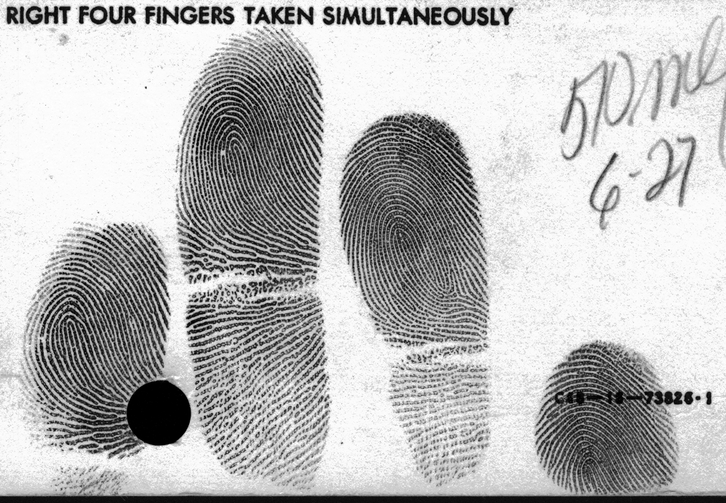
\includegraphics[width=0.49\linewidth]{images/a002-original}\hfill
  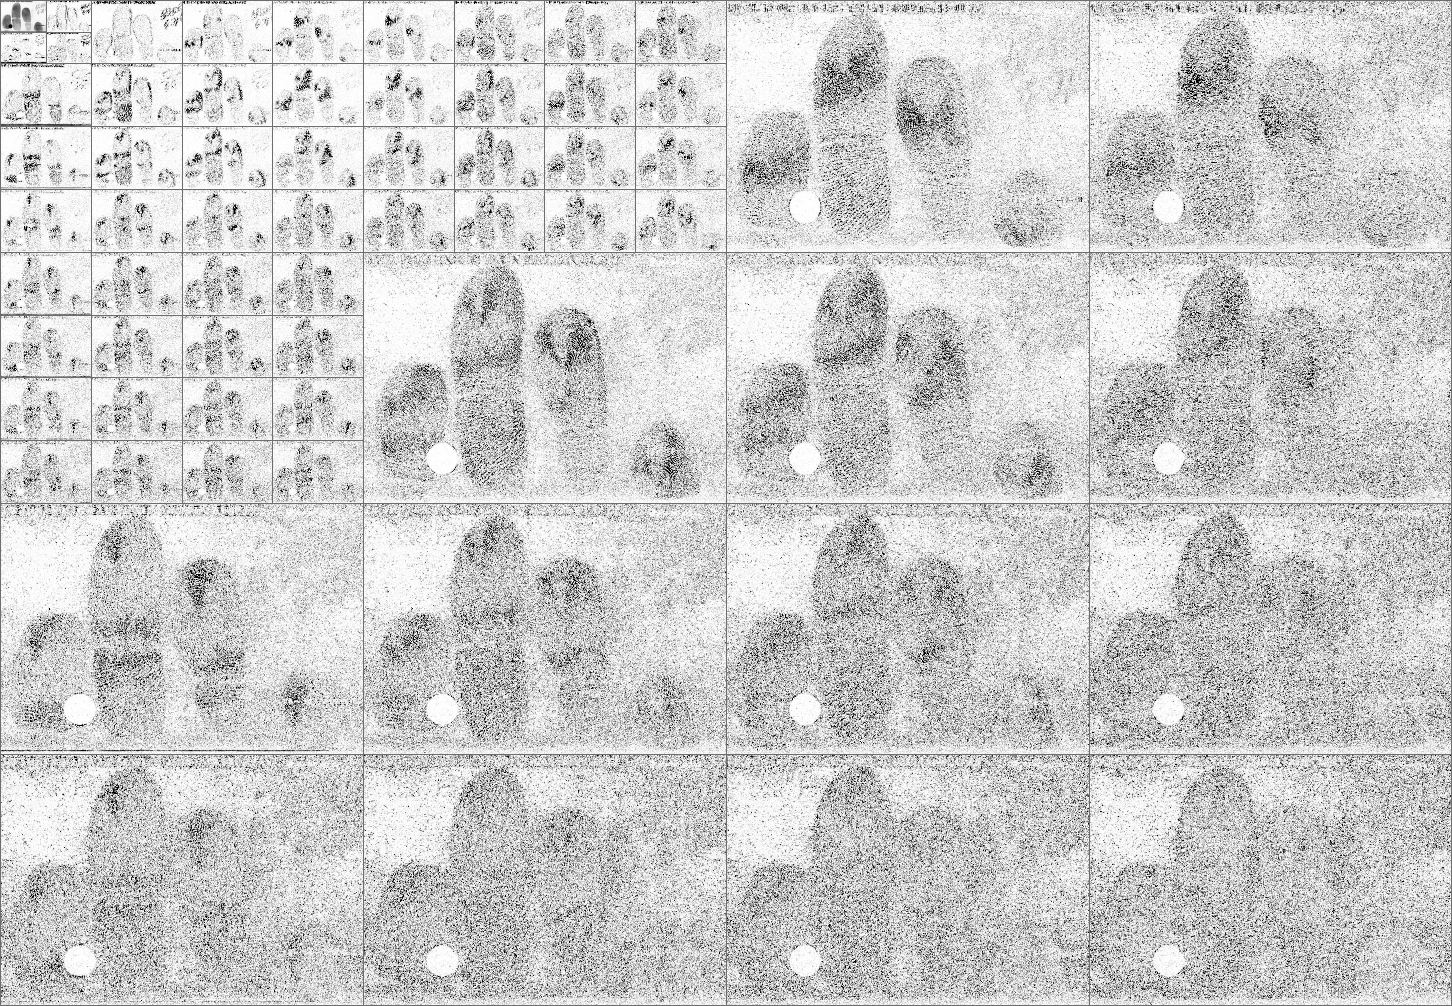
\includegraphics[width=0.49\linewidth]{images/a002-subbands}
  \caption{Image \texttt{a002} of the NIST compliance set ($1452 \times 1006$, a slap of four
  fingers) and its 64 subbands. Each subband is displayed with its own contrast (darker means
  a larger magnitude), except subband 0, which shows the coefficients themselves.}
  \label{fig:a002subbands}
\end{figure}
